\subsection{Experimental results}
This section contains experimental results to find the best possible price predicting solution. The results are divided into 5 experiments. The first experiment finds the best combination of input parameters for the network. These input parameters count meteorological, social and seasonal factors we identified in section~\ref{sec:Price}. The next experiment identifies the need for trimming and reasons why it is needed in this particular dataset. The third experiment tests different statistical strategies to incorporate historical prices as a part of the dataset. This includes historical prices, curve behavior analysis, skewness analysis and historical EWMA(Exponentially-Weighted Moving Average). The fourth experiment takes care of the Artificial Neural Network parameters. This includes black-box optimization like pruning of the network and optimization of epochs.

\subsubsection{Experiment 1: Inputs}
In this section we experimented with the basic input parameters that we identified in section~\ref{sec:Price}. We did a cross comparison of all the inputs and possible combinations (For those that made sense). The Price and the Demand is such a basic measure when you define a price in any markets that they are included in every prediction. We did not make a cross comparison of the Month of Year and the Seasons of Year since they say the same but with different granularity. We did a cross comparison both with and without matrix inputs and with a mix of non-matrix and matrix inputs. This is done to determine whether an input makes better sense on matrix form or just as a simple normalized value. 

Experiment 1 is based on a dataset consisting of the last 3 months averaging to about 2189 hours. We use 200 epochs for each training iteration.

This includes last hours Price (P), The Demand (D), Wind Speed(WS), Temperature(T), The Hourly Time of Day (ToD), The Day of The Week(DoW), The Month of The Year(MoY), The Season of The Year(SoY). The (M) is for Matrix input and states whether the input in the seasonal rows(ToD, WoD, MoY, SoY) are on matrix form or not.

As we saw in the wind production experiments(WPE) section~\ref{sec:windPowerAnalysis} there was a problem regarding the way we conducted tests for the seasonality; specifically for the MoY and the SoY. We only use the last 3 months to train the network and that sort of eliminates the obvious purpose of the MoY and SoY. As we saw in the results for the first experiment in WPE if we include the same month as we are in from last year and reintroduce the purpose of the SoY and MoY it gave us a worse result than leaving it out. To make sure the same thing applies on the price prediction experiments we conducted to runs of all the combinations of inputs. First we ran it with the last 3 months including the same month that we are in from last year and after that we ran the experiment with only the last 3 months.

Table~\ref{table:Top20Prices} shows us the top 20 MAE from the experiment with a training set containing the last 3 months(3Month). We have compared this to the experiment with a training set containing the last 3 months and the same month from last year(4Month). As we see in the table there isn't the biggest deviation between the two data sets. This also shows in \todo{Ref Appendix for both} that the distribution of the MAE over the two datasets are quite similar. From this we can conclude that the effect of using last years month in our dataset does not make a significant difference and can be left out. This raises the question if the MoY and the SoY can be left out as well, since the obvious use for it is eliminated by never having a full month or full season in the training set - that is equal to the one we predict.

First we conducted an experiment containing a training set with a full year (to test the effect of seasonality on a full year) we included the rest of the parameters equal to rank \#1 in table~\ref{table:Top20Prices} and shifted the seasonality. The results can be seen in table

\begin{table}[H]
\centering  % used for centering table
\resizebox{\textwidth}{!}{
\begin{tabular}{c c c c c c c c c c c c} % centered columns (7 columns)
P & D & WS & T & ToD & DoW & MoY & SoY & 3Month & 4Month Rank\\ [0.5ex] % inserts table 
%heading
\hline                  % inserts single horizontal line
 \x    & \x    & \x    & \x    & \x\m  & \x\m  &       & \x\m  & 57.12 & 61.70 & \#1 \\
 \x    & \x    & \x    & \x    & \x\m  & \x    &       & \x\m  & 58.09 & 68.23 & \#2 \\
 \x    & \x    & \x    & \x    & \x\m  &       & \x\m  &       & 58.79 & 63.80 & \#3 \\
 \x    & \x    & \x    &       & \x\m  & \x\m  & \x\m  &       & 60.14 & 67.82 & \#4 \\
 \x    & \x    & \x    & \x    & \x\m  & \x    &       &       & 62.19 & 74.89 & \#5 \\
 \x    & \x    & \x    & \x    & \x\m  &       &       & \x\m  & 62.26 & 61.86 & \#6 \\
 \x    & \x    & \x    & \x    & \x\m  & \x    & \x\m  &       & 62.84 & 62.62 & \#7 \\
 \x    & \x    & \x    & \x    & \x    & \x    &       & \x\m  & 63.94 & 72.37 & \#8 \\
 \x    & \x    & \x    & \x    & \x    & \x\m  & \x\m  &       & 64.19 & 84.12 & \#9 \\
 \x    & \x    & \x    &       & \x\m  & \x    & \x\m  &       & 64.72 & 72.29 & \#10 \\

 \x    & \x    & \x    &       & \x    & \x    & \x\m  &       & 65.07 & 79.71 & \#11 \\
 \x    & \x    & \x    & \x    & \x\m  & \x\m  &       &       & 65.95 & 58.19 & \#12 \\
 \x    & \x    & \x    & \x    & \x\m  & \x\m  & \x\m  &       & 66.55 & 67.31 & \#13 \\
 \x    & \x    & \x    &       & \x    &       &       & \x\m  & 67.21 & 74.67 & \#14 \\
 \x    & \x    & \x    & \x    & \x    & \x    &       &       & 67.88 & 77.29 & \#15 \\
 \x    & \x    & \x    &       & \x    & \x    &       & \x    & 68.21 & 72.45 & \#16 \\
 \x    & \x    & \x    &       & \x\m  & \x\m  &       &       & 68.34 & 72.31 & \#17 \\
 \x    & \x    & \x    &       & \x\m  &       &       & \x\m  & 68.35 & 76.25 & \#18 \\
 \x    & \x    & \x    & \x    & \x    & \x    & \x    &       & 68.43 & 75.10 & \#19 \\
 \x    & \x    & \x    & \x    & \x    &       &       & \x\m  & 68.45 & 75.97 & \#20 \\ \hline %inserts single line
\end{tabular}
}
\caption{The top 20 results on training set 3 last months} % title of Table
\label{table:Top20Prices} % is used to refer this table in the text
\end{table}

\begin{table}[H]
\centering  % used for centering table
\begin{tabular}{c c c c c c c c c c c} % centered columns (7 columns)
P & D & WS & T & ToD & DoW & MoY & SoY & MAE & Rank\\ [0.5ex] % inserts table 
\x    & \x    & \x    & \x    & \x\m  & \x\m  &       & \x\m  & 63.74 & \#1 \\
\x    & \x    & \x    & \x    & \x\m  & \x\m  &       &       & 90.79 & \#2 \\
\x    & \x    & \x    & \x    & \x\m  & \x\m  & \x\m  &       & 94.75 & \#3 \\
\end{tabular}
\caption{The top 20 results on training set 3 last months} % title of Table
\label{table:Top20Prices} % is used to refer this table in the text
\end{table}

If we take a look at the top 20 best input combinations shown in table~\ref{table:Top20Prices} we see some clear tendencies. If we start from the beginning the price and demand are static as mentioned earlier since they are fundamental market forces and thus not a changing factor in this analysis. The next input parameter is the Wind Speed. We see that every input combination in the top 20 includes the wind production and it is therefore a must for the prediction of the energy prices. This is further strengthened by the bottom 10 combinations table~\ref{table:Bottom10Prices} where we only see wind prices in one of the combinations. Also we saw in section~\ref{sec:windPowerAnalysis}(table~\ref{table:pearsonCoeficientWindProduction}) that the Wind Speed heavily influences the green energy production and thus influencing the energy prices. \todo{Lav en sammenligning af wind speed og wind production for at udelukke den ene}

The temperature is a less obvious candidate for the prediction of price since the Pearson's correlation between the two only are 0.17. Nevertheless it is showing up in 8/10 top combinations in table~\ref{table:Top20Prices} and this might be because of the correlation between temperature/demand which is -0.59. The temperature is scattered all over the 144 combinations and thus it is hard to say anything about this input with confidence. \todo{Lav en analyse med og uden temperatur paa den bedste}.

The Hourly Time of Day (ToD) is included in every single combination in the top 20. This clearly shows that this input parameter is important for the prediction of the price. This is kind of obvious since what we are predicting is the hourly price. In section~\ref{sec:seasonality}(figure~\ref{fig:price_per_hour}) we saw that the price varied from 190 to 335 which strengthens the importance of the relationship between time of day and the price. Also the top 7 all have the ToD on matrix form which indicates that this is the best way of representing the ToD.

Next we have the Day of the Week (DoW) parameter. This parameter are present in 75\% of the 20 best results (8/10 and in 15/20 best combinations). We have to believe that it plays a significant role in the prediction of price. If we look at the analysis of the average price over weekdays in section~\ref{sec:seasonality}(figure~\ref{fig:price_over_weekdays}) we see that there is a significant difference in price on the different days especially the weekdays compared to the weekend. This parameter is mixed between matrix input and standard input. This might be due to the fact that the biggest difference between days are weekend and weekday thus minimizing the effect of a matrix representation. \todo{Maaske lav et forsøg med weekday/weekend matrix.}

The last two parameters - Month of Year(MoY) and Season of Year (SoY) - are codependent and will be covered together. As mentioned before they cover the same information and we therefore only need one of them at any time \todo{Lav forsoeg der viser at det ikke giver mening at have baade MoY og SoY paa samme tid.}. The values are present in 9/10 of the best combinations in ~\ref{table:Top20Prices}. This is an indicator that the seasonality in the form of MoY and SoY plays a role in predicting the electricity price. Also we saw in the analysis in section~\ref{sec:seasonality}(figure~\ref{fig:monthlyAveragePrice} and ~\ref{fig:seasons}) that the price changes with seasonality and that it especially was more expensive in the winther than the rest of the year.


\begin{table}[H]
\centering  % used for centering table
\resizebox{\textwidth}{!}{
\begin{tabular}{c c c c c c c c c c c} % centered columns (7 columns)
P & D & WS & T & ToD & DoW & MoY & SoY & MAE & Rank\\ [0.5ex] % inserts table 
%heading
\hline                  % inserts single horizontal line
 \x    & \x    &       & \x    &       &       &       &       & 93.69 & \#132 \\
 \x    & \x    &       &       &       &       &       & \x    & 94.34 & \#133 \\
 \x    & \x    &       &       &       &       &       &       & 94.99 & \#134 \\
 \x    & \x    &       & \x    &       &       &       & \x\m  & 96.45 & \#135 \\
 \x    & \x    &       &       &       & \x\m  &       &       & 96.79 & \#136 \\
 \x    & \x    &       &       &       &       & \x\m  &       & 96.94 & \#137 \\
 \x    & \x    &       &       &       & \x    &       &       & 97.94 & \#138 \\
 \x    & \x    &       & \x    &       & \x\m  &       & \x\m  & 100.13 & \#139 \\
 \x    & \x    &       & \x    &       & \x\m  & \x\m  &       & 100.61 & \#140 \\
 \x    & \x    &       &       &       & \x\m  & \x\m  &       & 102.47 & \#141 \\
 \x    & \x    &       &       &       & \x    &       & \x    & 104.56 & \#142 \\
\end{tabular}
}
\caption{The bottom 10 input combinations for price prediction} % title of Table
\label{table:Bottom10Prices} % is used to refer this table in the text
\end{table}

If we take a look at the bottom 10 input combinations in terms of ability to predict the price we see some tendencies as well. 

%\begin{table}[H]
%\centering  % used for centering table
%\resizebox{\textwidth}{!}{
%	\begin{tabular}{c c c c c c c c c c c} % centered columns (7 columns)
%	P & D & WS & T & ToD & WoD & MoY & SoY & MAE & Rank\\ [0.5ex] % inserts table 
%	\hline                  % inserts single horizontal line
%	x & x & x & x & x    & x(M) & x(M) &      & 61,95 & \#1 \\ %newPredictions/TEN__MIXEDPrice_Consump_windSpeed_temperatureRow_timeOfDay_weekdaysMATRIX_monthOfYearMATRIX
%	x & x & x & x & x(M) & x    &      & x(M) & 62,76 & \#2 \\ %newPredictions/TEN__MIXEDPrice_Consump_windSpeed_temperatureRow_timeOfDayMATRIX_weekdays",%
%	x & x & x & x & x(M) & x(M) &      & x(M) & 62,87 & \#3 \\ %newPredictions/TEN__MIXEDPrice_Consump_windSpeed_temperatureRow_timeOfDayMATRIX_weekdays_monthOfYearMATRIX",
%	x & x & x &   & x(M) & x    & x(M) &      & 62,99 & \#4 \\ %newPredictions/TEN__MIXEDPrice_Consump_windSpeed_timeOfDayMATRIX_weekdays_monthOfYearMATRIX",
%	x & x & x & x & x(M) & x    & x(M) &      & 64,24 & \#5 \\ %newPredictions/TEN__MATRIX_Price_Consump_windSpeed_temperatureRow_timeOfDay_weekdays_seasonOfYear",
%	x & x & x & x & x(M) & x    &      &      & 65,18 & \#6 \\ %newPredictions/TEN__MIXEDPrice_Consump_windSpeed_temperatureRow_timeOfDayMATRIX_weekdays_seasonOfYearMATRIX",
%	x & x & x & x & x(M) &      & x(M) &      & 65,53 & \#7 \\ %newPredictions/TEN__MIXEDPrice_Consump_windSpeed_temperatureRow_timeOfDayMATRIX_monthOfYearMATRIX",
%	x & x & x & x & x    & x    &      & x(M) & 65,80 & \#8 \\ %newPredictions/TEN__MIXEDPrice_Consump_windSpeed_temperatureRow_timeOfDayMATRIX_seasonOfYearMATRIX",
%	x & x & x & x & x(M) &      &      & x(M) & 67,21 & \#9 \\ %newPredictions/TEN__MIXEDPrice_Consump_windSpeed_temperatureRow_timeOfDay_weekdays_seasonOfYearMATRIX",
%	x & x & x &   & x(M) & x(M) & x(M) &      & 70,25 & \#10 \\ %newPredictions/TEN__MATRIX_Price_Consump_windSpeed_timeOfDay_weekdays_monthOfYear"
%	\hline %inserts single line
%	\end{tabular}
%}
%\caption{Average MAE of ten runs per entry} % title of Table
%\label{table:Top10Average} % is used to refer this table in the text
%\end{table}

\subsubsection{Experiment 2: Trimming}
\begin{figure}[H]
\centering
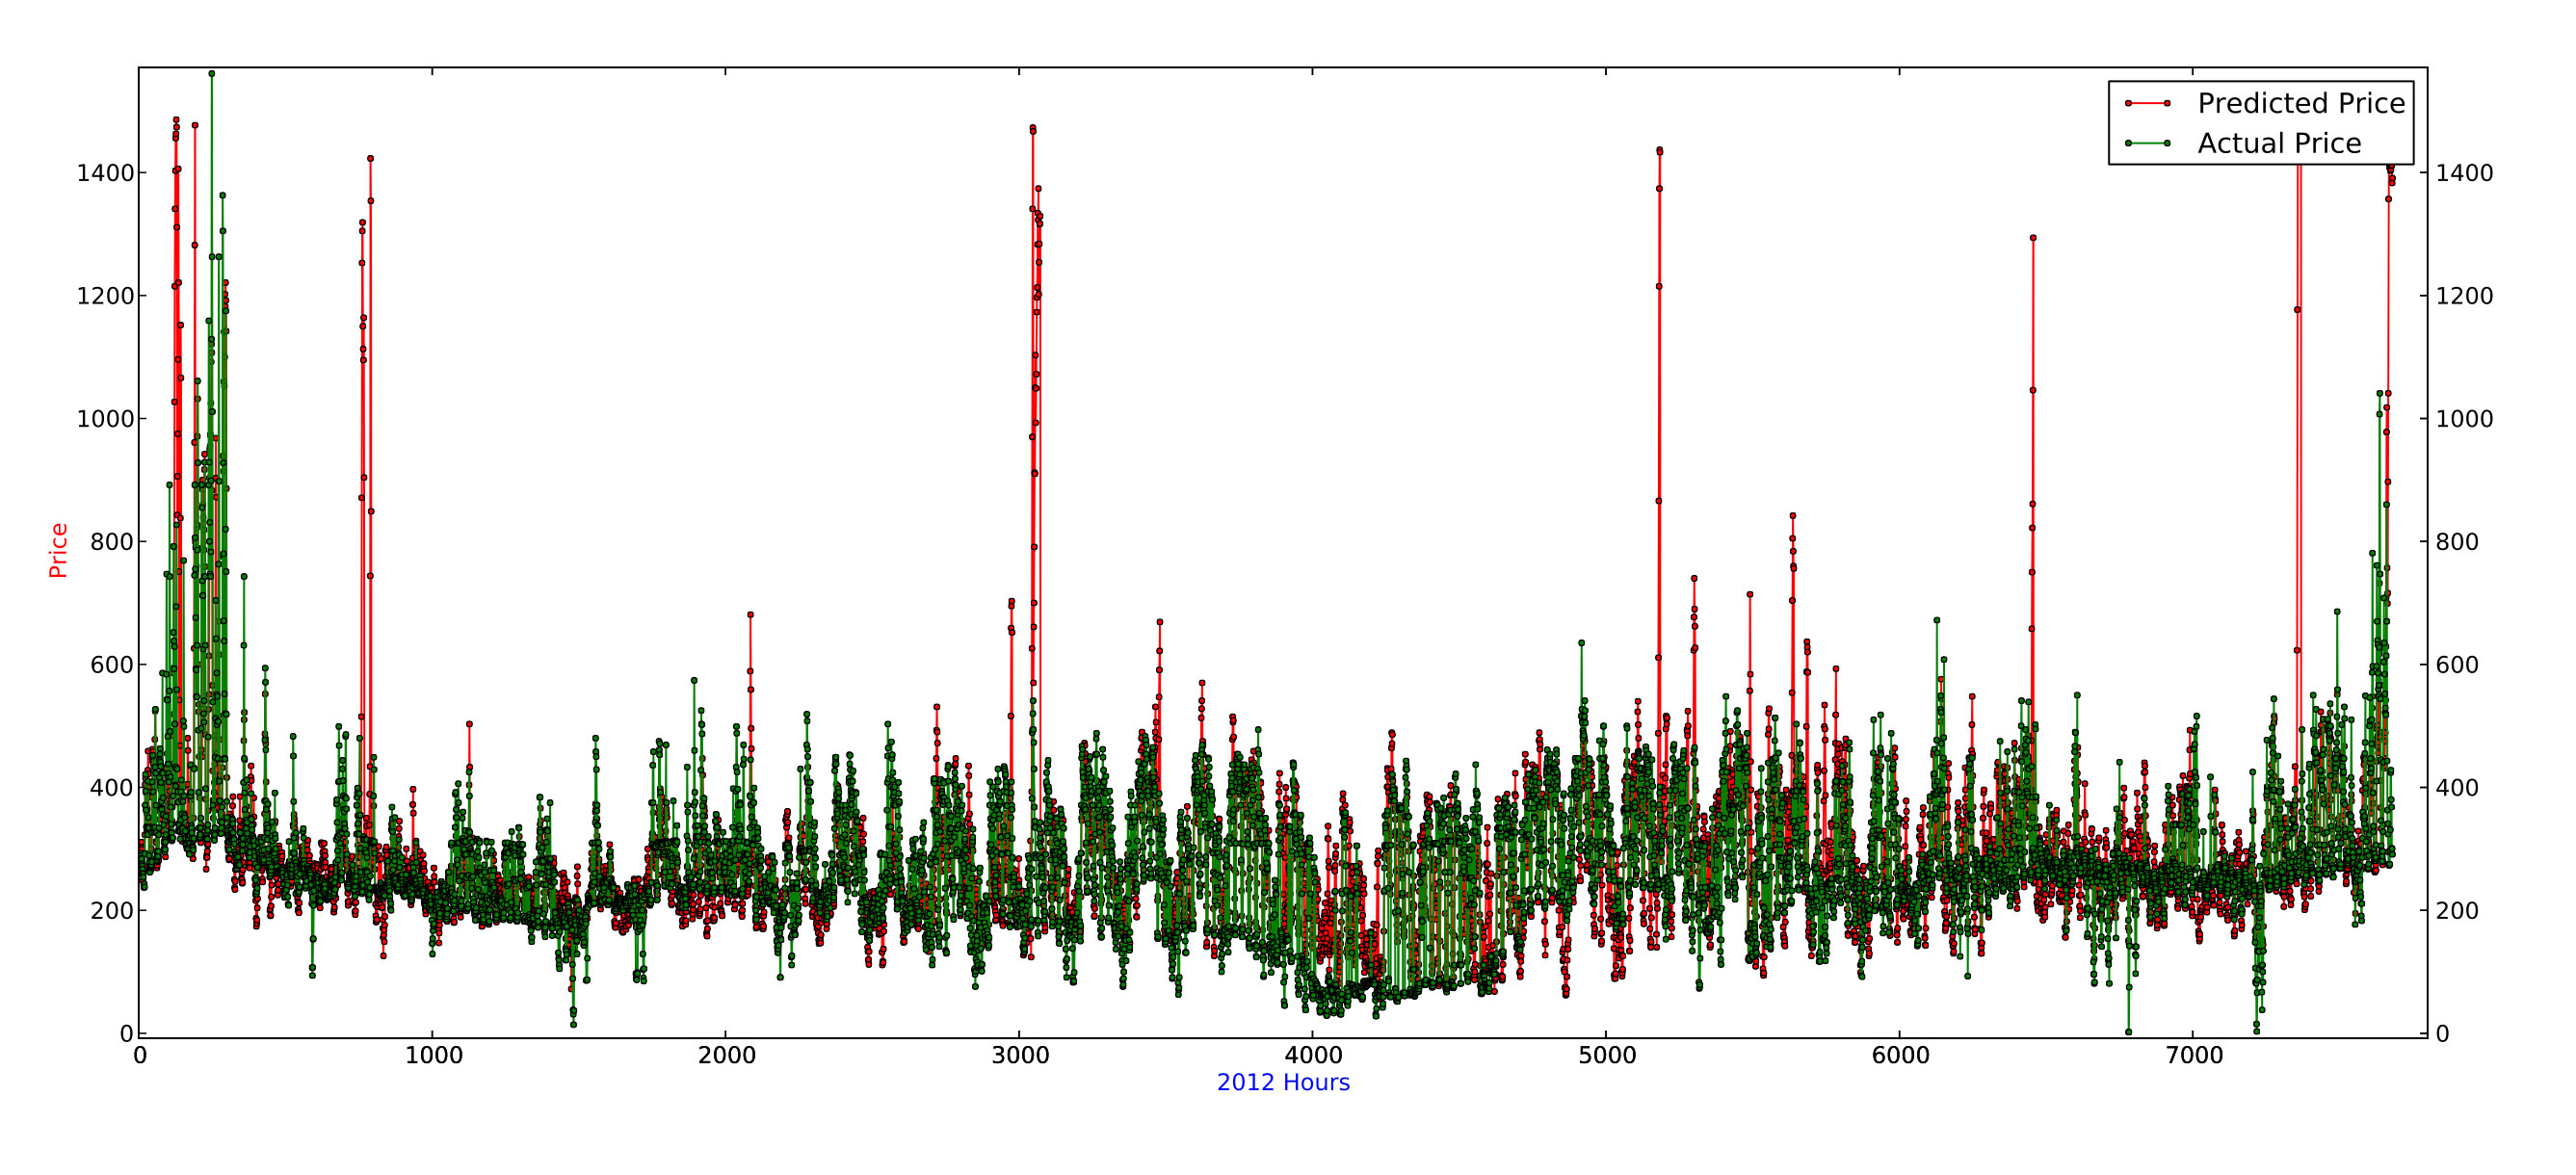
\includegraphics[width=0.85\linewidth,natwidth=898,natheight=587]{billeder/PriceExperimentalAnalysis/NoTrimming.jpg}
\caption{The \#1 forecast with no trimming of the dataset}
\label{fig:NoTrim}
\end{figure}

\begin{figure}[H]
\centering
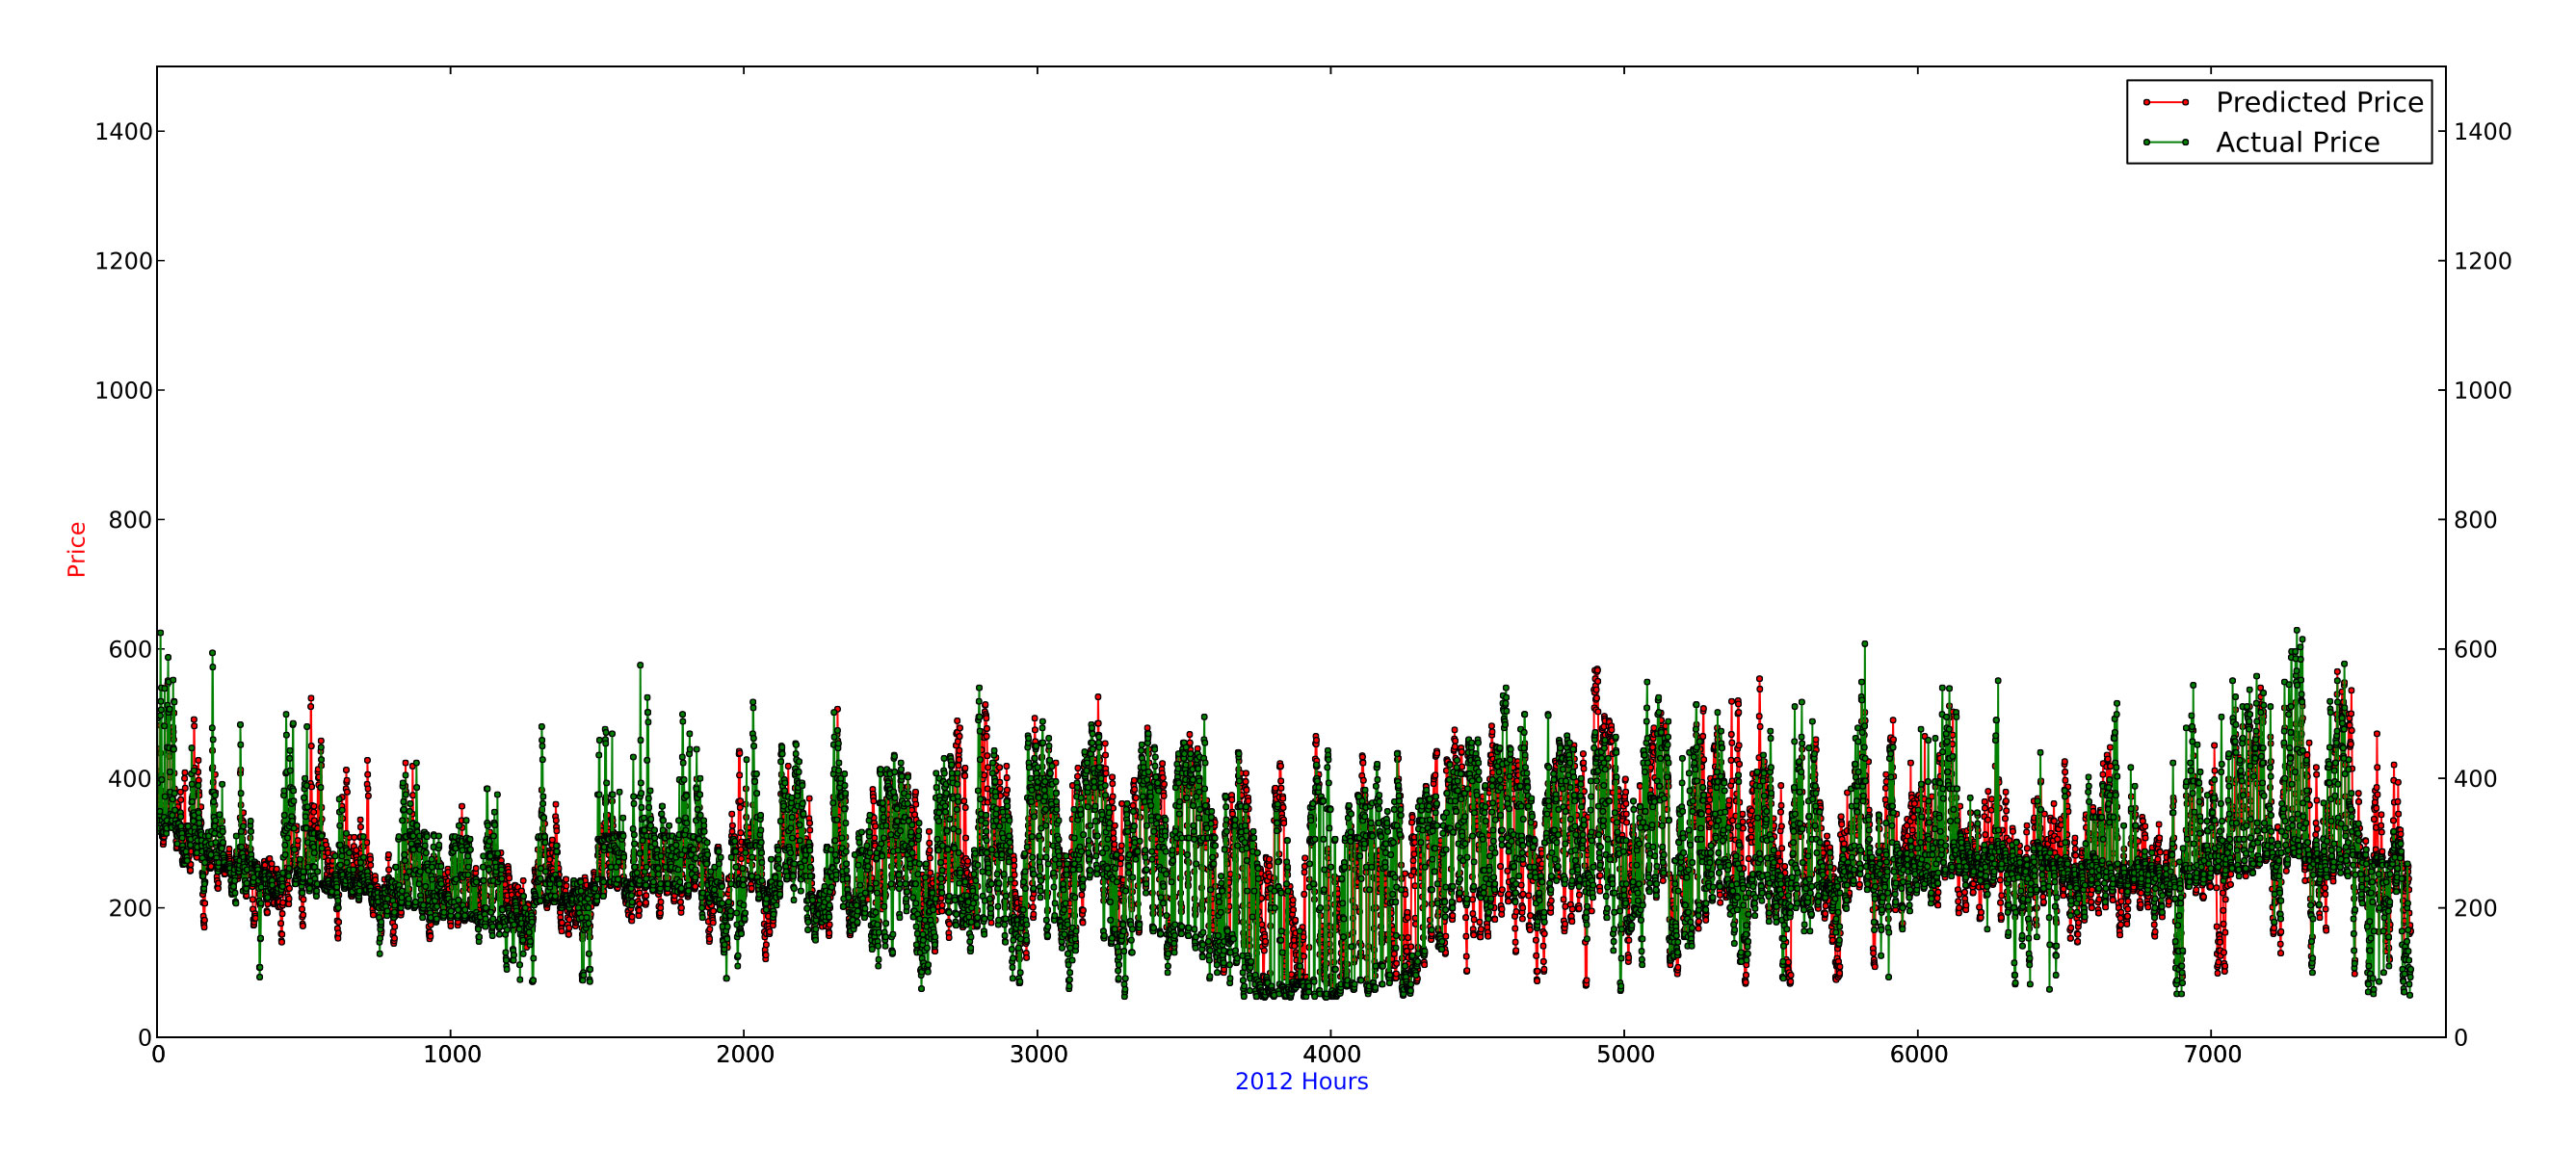
\includegraphics[width=0.85\linewidth,natwidth=898,natheight=587]{billeder/PriceExperimentalAnalysis/1PTrim.jpg}
\caption{The \#1 forecast with 1\% trimming in both ends of the dataset}
\label{fig:1PTrim}
\end{figure}

\begin{table}[H]
\centering  % used for centering table
\resizebox{0.6\textwidth}{!}{
	\begin{tabular}{c c c c c c} % centered columns (7 columns)
	1PTrim & 2PTrim & 3PTrim & 4PTrim & 5PTrim & Number\\ [0.5ex] % inserts table 
	\hline                  % inserts single horizontal line
	47,21 & 42,90 & 44,48 & 42,46 & 41,79 & \#1 \\
	46,15 & 43,67 & 43,07 & 39,16 & 40,28 & \#2 \\
	47,14 & 45,10 & 43,38 & 40,50 & 39,41 & \#3 \\
	46,70 & 43,96 & 43,21 & 40,03 & 40,29 & \#4 \\
	45,96 & 43,25 & 45,51 & 40,74 & 40,42 & \#5 \\
	47,27 & 45,96 & 44,98 & 41,39 & 39,98 & \#6 \\
	45,93 & 44,66 & 43,39 & 41,02 & 40,40 & \#7 \\
	46,64 & 42,69 & 44,48 & 41,69 & 40,61 & \#8 \\
	45,98 & 44,51 & 43,71 & 40,74 & 41,08 & \#9 \\
	45,60 & 46,07 & 45,81 & 42,52 & 41,32 & \#10 \\
	\hline %inserts single line
	\end{tabular}
}
\caption{Trims} % title of Table
\label{table:Top10Trimming} % is used to refer this table in the text
\end{table}

363 entries gets removed per percent.

\subsubsection{Experiment 3: Statistical strategies}

\subsubsection{Experiment 4: Black box optimization}

